\chapter{Pola Kreasi (Bagian 2)}

\section{Pola Kreasi: Builder}

\subsection{Tujuan dan Konteks Penggunaan}

Pola \textit{Builder} merupakan salah satu pola kreasi yang bertujuan untuk memisahkan konstruksi sebuah objek kompleks dari representasinya, sehingga proses yang sama dapat digunakan untuk membuat berbagai representasi objek. Pola ini sangat berguna ketika proses pembuatan suatu objek melibatkan banyak langkah, parameter opsional, atau struktur bersarang yang kompleks, dan sulit dikelola hanya dengan konstruktor biasa atau metode \texttt{setter}.

Tujuan utama dari pola Builder adalah untuk mengatasi masalah kompleksitas dalam instansiasi objek, terutama ketika:
\begin{itemize}
\item Objek memiliki banyak atribut opsional atau konfigurasi berbeda.
\item Proses pembuatan objek membutuhkan urutan langkah tertentu.
\item Dibutuhkan pemisahan antara bagaimana sebuah objek dikonstruksi dan seperti apa hasil akhirnya.
\end{itemize}

Pola ini biasanya digunakan dalam sistem yang perlu membuat objek dengan struktur hierarkis atau dengan banyak komponen, di mana tiap bagian dapat dibangun secara terpisah namun dikombinasikan dalam satu kesatuan.

Pola Builder sering ditemukan dalam situasi seperti:
\begin{itemize}
\item Pembuatan dokumen (misalnya PDF, HTML) yang memiliki banyak bagian dan layout.
\item Konstruksi objek \texttt{Product} dari berbagai bagian seperti \texttt{PartA}, \texttt{PartB}, dan \texttt{PartC}.
\item Pembuatan objek konfigurasi kompleks, seperti koneksi database atau objek HTTP request dengan banyak parameter.
\end{itemize}

Pola ini juga populer dalam pengembangan API yang mendukung gaya pemrograman \textit{fluent interface}, karena memudahkan pembacaan dan penulisan kode dengan cara chaining method secara bertahap saat membangun sebuah objek.

\subsection{Contoh Kasus Penggunaan}

Salah satu contoh klasik penggunaan pola \textit{Builder} adalah dalam pembuatan objek yang kompleks seperti \texttt{Meal} pada sistem pemesanan makanan cepat saji. Objek \texttt{Meal} dapat terdiri dari berbagai komponen seperti makanan utama, minuman, makanan penutup, dan tambahan lain, yang dapat dikombinasikan dalam berbagai variasi. Dengan pola \textit{Builder}, setiap variasi menu dapat dibuat menggunakan proses yang sama, tetapi dengan hasil akhir yang berbeda.

Contoh lainnya adalah pada pembuatan dokumen atau laporan yang terdiri dari banyak bagian seperti judul, header, isi, footer, dan lampiran. Masing-masing bagian bisa dibangun terpisah, kemudian digabungkan menjadi dokumen lengkap oleh objek \texttt{Builder}.

Pola ini juga umum digunakan dalam pembuatan objek konfigurasi kompleks, misalnya saat membangun objek \texttt{HttpRequest} dalam sebuah pustaka HTTP. Karena banyak parameter seperti URL, header, metode, isi permintaan, dan autentikasi bersifat opsional, maka lebih efisien menggunakan pola \textit{Builder} daripada menyediakan berbagai konstruktor untuk setiap kombinasi parameter.

\textbf{Contoh dalam praktik:}
\begin{itemize}
\item Dalam framework seperti \texttt{StringBuilder} di Java, di mana string dibangun secara bertahap tanpa membuat objek string baru setiap saat.
\item Pada pustaka seperti \texttt{Jackson} atau \texttt{Gson} yang menyediakan builder untuk menyusun objek serialisasi/deserialisasi JSON.
\item Dalam pengembangan antarmuka pengguna (UI), builder dapat digunakan untuk menyusun tampilan layar dengan komponen yang kompleks seperti tombol, formulir, dan tabel, yang masing-masing memiliki konfigurasi berbeda.
\end{itemize}

Dengan menggunakan pola \textit{Builder}, sistem menjadi lebih fleksibel dalam membuat objek dengan berbagai konfigurasi, serta lebih mudah dibaca dan dipelihara karena kode pembuatan objek disusun secara deklaratif dan bertahap.


\subsection{Kelebihan dan Kekurangan}

\textbf{Kelebihan:}
\begin{itemize}
\item \textbf{Mengelola kompleksitas objek secara efisien:} Pola Builder memungkinkan pembuatan objek yang kompleks dengan banyak atribut atau komponen secara bertahap, tanpa harus membuat konstruktor dengan parameter yang panjang atau membingungkan.

\item \textbf{Mendukung prinsip Single Responsibility:} Proses pembuatan objek dipisahkan dari representasinya, sehingga kelas produk (misalnya \texttt{Car}, \texttt{Meal}) hanya fokus pada perilaku, sementara logika konstruksi didelegasikan ke kelas builder.

\item \textbf{Mendukung chaining dan fluent interface:} Builder memungkinkan pemrogram menulis kode yang lebih bersih dan mudah dibaca menggunakan pola method chaining seperti \texttt{build\-er.set\-A().setB().build()}.

\item \textbf{Fleksibel terhadap perubahan:} Menambahkan, menghapus, atau mengubah bagian dari proses pembuatan objek lebih mudah dilakukan tanpa harus mengubah antarmuka klien atau konstruktor.

\item \textbf{Meningkatkan keterbacaan kode:} Karena konfigurasi objek dibangun secara eksplisit dan bertahap, pengembang dapat dengan mudah memahami struktur dan isi objek tanpa harus menelusuri banyak konstruktor.
\end{itemize}

\textbf{Kekurangan:}
\begin{itemize}
\item \textbf{Menambah jumlah kelas:} Untuk setiap jenis produk kompleks, perlu dibuat satu kelas \texttt{Builder} tambahan, yang dapat meningkatkan jumlah file dan kompleksitas struktur kode.

\item \textbf{Kurang cocok untuk objek sederhana:} Untuk objek yang hanya memiliki sedikit atribut atau konfigurasi, pola Builder dianggap berlebihan dan justru memperumit kode.

\item \textbf{Potensi duplikasi logika:} Jika tidak dirancang dengan baik, bisa terjadi duplikasi antara logika validasi atau inisialisasi di kelas produk dan di kelas builder.

\item \textbf{Kesalahan urutan pemanggilan:} Jika tidak digunakan dengan hati-hati, pola Builder bisa menyebabkan objek yang dihasilkan tidak valid jika urutan pemanggilan metode builder tidak sesuai atau ada langkah yang terlewat.
\end{itemize}


\subsection{Implementasi dalam Java}

Implementasi pola \textit{Builder} dalam Java dapat divisualisasikan seperti yang ditunjukkan pada Gambar~\ref{fig:builder}. Diagram tersebut menggambarkan bagaimana sebuah kelas produk (\texttt{Computer}) dipisahkan dari kelas \texttt{Builder} yang bertanggung jawab atas proses pembuatannya. Pola ini memungkinkan proses konstruksi objek dilakukan secara bertahap dengan menyediakan metode-metode konfigurasi sebelum akhirnya membangun objek final. Berikut ini adalah contoh implementasi kode dalam Java yang sesuai dengan struktur tersebut.

\begin{figure}[h]
 	\centering
 	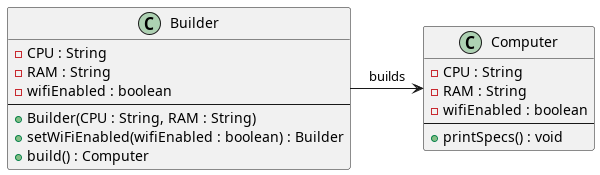
\includegraphics[width=.9\textwidth]{../figures/out/builder.png}
 	\caption{Builder Pattern}
 	\label{fig:builder}
\end{figure}


\subsection{Contoh Computer Builder}

\begin{lstlisting}[style=JavaStyle, caption={Implementasi Builder pada Kelas Computer}, label={lst:builder-computer}]
public class Computer {
	private String CPU;     // wajib
	private String RAM;     // wajib
	private String storage; // opsional
	
	private Computer(Builder builder) {
		this.CPU = builder.CPU;
		this.RAM = builder.RAM;
		this.storage = builder.storage;
	}
	
	public void printSpecs() {
		System.out.println("CPU: " + CPU);
		System.out.println("RAM: " + RAM);
		System.out.println("Storage: " + storage);
	}
	
	public static class Builder {
		private String CPU;
		private String RAM;
		private String storage;
		
		public Builder(String CPU, String RAM) {
			this.CPU = CPU;
			this.RAM = RAM;
		}
		
		public Builder setStorage(String storage) {
			this.storage = storage;
			return this;
		}
		
		public Computer build() {
			return new Computer(this);
		}
	}
}
\end{lstlisting}

Kode di atas mengimplementasikan pola \textit{Builder} untuk membangun objek \texttt{Computer} yang memiliki dua atribut wajib, yaitu \texttt{CPU} dan \texttt{RAM}, serta satu atribut opsional, yaitu \texttt{storage}. 

Kelas \texttt{Computer} memiliki konstruktor privat yang menerima objek \texttt{Builder} sebagai parameter. Di dalam konstruktor ini, semua atribut \texttt{Computer} diisi menggunakan nilai yang diberikan oleh \texttt{Builder}. Dengan pendekatan ini, pembuatan objek \texttt{Computer} tidak dilakukan secara langsung, melainkan melalui objek \texttt{Builder}.

Kelas \texttt{Builder} adalah kelas statis dalam \texttt{Computer} yang bertugas untuk membangun instansi \texttt{Computer}. Kelas ini menyediakan konstruktor yang memerlukan dua parameter wajib, yaitu \texttt{CPU} dan \texttt{RAM}, serta metode opsional \texttt{setStorage(String storage)} untuk menetapkan nilai \texttt{storage}. Metode \texttt{setStorage} mengembalikan dirinya sendiri sehingga memungkinkan penggunaan \textit{method chaining}. Metode \texttt{build()} akan memanggil konstruktor privat \texttt{Computer} dan mengembalikan objek hasil pembangunan.

Pola ini memungkinkan pengembang untuk membangun objek \texttt{Computer} secara bertahap dan fleksibel. Sebagai contoh, klien dapat memilih untuk mengatur \texttt{storage} atau tidak, tanpa harus membuat banyak konstruktor berbeda. Hal ini membuat kode lebih bersih, modular, dan mudah dipelihara, terutama jika jumlah atribut opsional bertambah di masa depan.

Selain itu, implementasi ini mendukung prinsip \textit{Single Responsibility}, karena logika pembuatan objek dipisahkan dari perilaku fungsional objek \texttt{Computer} itu sendiri.


\begin{lstlisting}[style=JavaStyle, caption={Penggunaan Builder untuk Membuat Objek Computer}, label={lst:builder-main}]
public class Main {
	public static void main(String[] args) {
		Computer pc1 = new Computer.Builder("Intel i5", "8GB")
		.setStorage("512GB SSD")
		.build();
		
		pc1.printSpecs();
		
		Computer pc2 = new Computer.Builder("AMD Ryzen 5", "16GB")
		.build();
		
		pc2.printSpecs();
	}
}
\end{lstlisting}

Kode di atas menunjukkan bagaimana pola \textit{Builder} digunakan untuk membuat dua objek \texttt{Computer} dengan konfigurasi yang berbeda. Pada objek pertama, \texttt{pc1}, builder dipanggil dengan menetapkan \texttt{CPU} "Intel i5" dan \texttt{RAM} "8GB", kemudian menambahkan atribut opsional \texttt{storage} sebesar "512GB SSD" sebelum akhirnya memanggil metode \texttt{build()} untuk menghasilkan objek \texttt{Computer} yang lengkap.

Objek kedua, \texttt{pc2}, dibangun hanya dengan \texttt{CPU} "AMD Ryzen 5" dan \texttt{RAM} "16GB" tanpa menetapkan atribut \texttt{storage}, sehingga nilai \texttt{storage} akan tetap \texttt{null} atau kosong sesuai implementasi di dalam kelas \texttt{Computer}.

Setelah masing-masing objek dibuat, metode \texttt{printSpecs()} dipanggil untuk menampilkan spesifikasi komputer ke konsol. Contoh ini menunjukkan fleksibilitas pola \textit{Builder}, di mana atribut opsional dapat diatur atau diabaikan sesuai kebutuhan tanpa membuat kode menjadi berantakan atau sulit dibaca.


\section{Contoh Ticket Order}

\begin{lstlisting}[style=JavaStyle, caption={Implementasi Builder pada Kelas TicketOrder}, label={lst:builder-ticket}]
public class TicketOrder {
	private String eventName;   // wajib
	private String seatNumber;  // wajib
	private boolean withMeal;   // opsional
	
	private TicketOrder(Builder builder) {
		this.eventName = builder.eventName;
		this.seatNumber = builder.seatNumber;
		this.withMeal = builder.withMeal;
	}
	
	public void printOrder() {
		System.out.println("Event: " + eventName);
		System.out.println("Seat: " + seatNumber);
		System.out.println("Meal Included: " + withMeal);
	}
	
	public static class Builder {
		private String eventName;
		private String seatNumber;
		private boolean withMeal = false; // default
		
		public Builder(String eventName, String seatNumber) {
			this.eventName = eventName;
			this.seatNumber = seatNumber;
		}
		
		public Builder setWithMeal(boolean withMeal) {
			this.withMeal = withMeal;
			return this;
		}
		
		public TicketOrder build() {
			return new TicketOrder(this);
		}
	}
}
\end{lstlisting}

Kode di atas mengimplementasikan pola \textit{Builder} untuk membangun objek \texttt{TicketOrder} yang merepresentasikan pesanan tiket suatu acara. Objek \texttt{TicketOrder} memiliki dua atribut wajib, yaitu \texttt{eventName} dan \texttt{seatNumber}, serta satu atribut opsional berupa \texttt{withMeal} yang menunjukkan apakah pemesan memilih tambahan layanan makan.

Konstruktor kelas \texttt{TicketOrder} bersifat privat dan menerima sebuah objek \texttt{Builder}. Nilai-nilai atribut diambil dari atribut builder tersebut. Dengan pendekatan ini, pembuatan objek \texttt{TicketOrder} dikendalikan sepenuhnya melalui kelas \texttt{Builder}.

Kelas \texttt{Builder} sebagai kelas statis di dalam \texttt{TicketOrder} menyediakan konstruktor yang mensyaratkan pengisian \texttt{eventName} dan \texttt{seatNumber} saat instansiasi. Selain itu, tersedia metode opsional \texttt{setWithMeal(boolean withMeal)} yang memungkinkan pemesan memilih apakah layanan makan akan disertakan. Metode ini mendukung \textit{method chaining} dengan mengembalikan dirinya sendiri. Metode \texttt{build()} digunakan untuk menghasilkan instansi \texttt{TicketOrder} berdasarkan nilai-nilai yang sudah diatur pada builder.

Pola ini memberikan fleksibilitas dalam membangun objek \texttt{TicketOrder} dengan atau tanpa tambahan layanan makan tanpa harus membuat konstruktor yang berisi semua kemungkinan kombinasi parameter. Struktur ini juga mendukung keterbacaan kode, modularitas, dan mempermudah pemeliharaan sistem di masa depan.

\begin{lstlisting}[style=JavaStyle, caption={Penggunaan Builder untuk Membuat Pesanan Tiket}, label={lst:builder-ticket-main}]
public class Main {
	public static void main(String[] args) {
		TicketOrder order1 = new TicketOrder.Builder("Concert A", "A12")
		.setWithMeal(true)
		.build();
		
		order1.printOrder();
		
		TicketOrder order2 = new TicketOrder.Builder("Theatre B", "B25")
		.build();
		
		order2.printOrder();
	}
}
\end{lstlisting}

Kode di atas menunjukkan bagaimana pola \textit{Builder} digunakan untuk membuat dua objek \texttt{TicketOrder} dengan konfigurasi yang berbeda. Pada objek pertama, \texttt{order1}, builder dipanggil dengan menentukan nama acara "Concert A" dan nomor kursi "A12", kemudian menambahkan layanan makan (\texttt{withMeal = true}) sebelum akhirnya membangun objek dengan memanggil metode \texttt{build()}.

Objek kedua, \texttt{order2}, dibuat hanya dengan nama acara "Theatre B" dan nomor kursi "B25" tanpa menambahkan layanan makan, sehingga atribut \texttt{withMeal} akan tetap bernilai \texttt{false} sesuai nilai default yang telah ditentukan pada kelas \texttt{Builder}.

Setelah masing-masing objek pesanan tiket dibuat, metode \texttt{printOrder()} dipanggil untuk menampilkan informasi pesanan ke konsol. Contoh ini memperlihatkan bagaimana pola \textit{Builder} memberikan fleksibilitas dalam menentukan atribut opsional tanpa membuat kode menjadi rumit, serta memungkinkan pemanggilan metode secara berantai untuk meningkatkan keterbacaan.

\section{Pola Kreasi: Prototype}

\subsection{Tujuan dan Konteks Penggunaan}

Pola \textit{Prototype} adalah salah satu pola kreasi yang bertujuan untuk membuat objek baru dengan menyalin atau menduplikasi objek yang sudah ada, bukan dengan membuatnya dari awal menggunakan konstruktor. Pendekatan ini sangat berguna ketika pembuatan objek baru membutuhkan biaya besar dalam hal waktu, sumber daya, atau konfigurasi yang kompleks.

Tujuan utama dari pola \textit{Prototype} adalah untuk:
\begin{itemize}
\item Mengurangi biaya pembuatan objek yang mahal, baik dalam hal performa maupun kompleksitas struktur.
\item Menyederhanakan proses pembuatan objek dengan menggunakan salinan dari objek yang sudah terdefinisi.
\item Memberikan fleksibilitas dalam membuat berbagai variasi objek berdasarkan template dasar tanpa bergantung pada kelas konkret atau logika pembuatan yang rumit.
\end{itemize}

Pola ini biasanya diimplementasikan dengan menyediakan metode \texttt{clone()} pada kelas objek, yang bertugas mengembalikan salinan dari objek itu sendiri. Terdapat dua pendekatan dalam implementasi cloning, yaitu:
\begin{itemize}
\item \textbf{Shallow copy}: Menyalin nilai atribut dasar, namun referensi ke objek lain tetap mengarah ke objek yang sama.
\item \textbf{Deep copy}: Menyalin seluruh struktur objek termasuk objek-objek yang direferensikan, sehingga menghasilkan salinan yang sepenuhnya independen dari objek asal.
\end{itemize}

Pola \textit{Prototype} sangat berguna dalam situasi seperti:
\begin{itemize}
\item Ketika ada banyak konfigurasi serupa dan hanya beberapa atribut kecil yang berbeda.
\item Ketika objek yang sama perlu dibuat berkali-kali dengan pengaturan awal yang identik.
\item Saat diperlukan pembuatan objek baru dengan cepat di runtime tanpa bergantung pada logika instansiasi kelas.
\end{itemize}

Dengan menggunakan pola ini, sistem menjadi lebih fleksibel, hemat sumber daya, dan lebih mudah dalam mengelola variasi objek yang kompleks.


\subsection{Contoh Kasus Penggunaan}

Salah satu contoh umum penggunaan pola \textit{Prototype} adalah dalam sistem pembuatan karakter dalam permainan video (game). Saat pemain membuat karakter baru, sistem dapat menduplikasi template karakter dasar seperti \texttt{Warrior}, \texttt{Mage}, atau \texttt{Archer} dan kemudian mengubah atribut spesifik seperti warna rambut, pakaian, atau kemampuan, tanpa harus membangun karakter dari awal.

Contoh lainnya adalah dalam aplikasi desain grafis, di mana pengguna dapat membuat duplikasi elemen grafis seperti bentuk, ikon, atau komponen UI. Daripada membuat ulang setiap elemen dari awal, pengguna dapat mengkloning elemen yang sudah ada dan memodifikasinya sesuai kebutuhan.

Di dunia bisnis, pola ini digunakan dalam sistem manajemen dokumen atau laporan, di mana template dokumen standar dapat dikloning dan disesuaikan untuk masing-masing proyek atau klien. Dengan cara ini, konsistensi format tetap terjaga sambil memungkinkan personalisasi isi.

Contoh tambahan yang lebih teknis adalah dalam sistem konfigurasi atau pengaturan. Misalnya, sebuah aplikasi memiliki objek konfigurasi default yang dapat dikloning untuk pengguna baru, sehingga pengguna dapat memiliki konfigurasi awal yang dapat diubah tanpa mempengaruhi template konfigurasi dasar.

Dengan pola \textit{Prototype}, pembuatan objek menjadi lebih efisien dan konsisten, terutama saat berurusan dengan objek yang memiliki struktur kompleks atau pengaturan default yang umum digunakan.


\subsection{Kelebihan dan Kekurangan}

\textbf{Kelebihan:}
\begin{itemize}
\item \textbf{Menghemat waktu dan sumber daya:} Pembuatan objek baru dengan menyalin objek yang sudah ada lebih cepat dibandingkan membangun dari awal, terutama untuk objek kompleks atau yang memiliki banyak konfigurasi.

\item \textbf{Meningkatkan konsistensi:} Dengan menggunakan objek prototipe sebagai dasar, sistem dapat memastikan bahwa semua objek baru memiliki struktur dan nilai default yang seragam.

\item \textbf{Mendukung pembuatan dinamis di runtime:} Pola ini memungkinkan penciptaan objek baru selama program berjalan tanpa harus bergantung pada logika konstruktor atau pengetahuan tentang kelas konkret.

\item \textbf{Mempermudah pembuatan variasi objek:} Modifikasi kecil dapat dilakukan pada salinan prototipe tanpa mempengaruhi objek asli, sehingga mendukung fleksibilitas dalam mengelola perbedaan antar objek.

\item \textbf{Mengurangi ketergantungan antar kelas:} Kode klien tidak perlu mengetahui bagaimana objek dibuat; cukup meminta salinan dari prototipe yang ada.
\end{itemize}

\textbf{Kekurangan:}
\begin{itemize}
\item \textbf{Kesulitan dalam implementasi cloning yang kompleks:} Jika objek memiliki struktur dalam (nested object) atau hubungan antarobjek, maka implementasi \textit{deep copy} bisa menjadi rumit dan rawan kesalahan.

\item \textbf{Potensi kesalahan akibat shallow copy:} Jika hanya menggunakan salinan dangkal (\textit{shallow copy}), perubahan pada objek salinan dapat berdampak pada objek asli jika mereka berbagi referensi ke objek lain.

\item \textbf{Sulit diterapkan pada objek yang tidak mendukung cloning:} Tidak semua objek mudah atau aman untuk dikloning, terutama jika terdapat sumber daya eksternal seperti koneksi jaringan, file sistem, atau sesi database.

\item \textbf{Meningkatkan kompleksitas debugging:} Ketika banyak salinan objek tersebar di sistem, melacak asal-usul perubahan data atau bug bisa menjadi lebih sulit.

\item \textbf{Ketergantungan terhadap implementasi clone:} Jika metode \texttt{clone()} tidak diimplementasikan dengan benar di semua kelas terkait, hasil cloning bisa menyebabkan inkonsistensi atau error tersembunyi.
\end{itemize}


\subsection{Implementasi dalam Java}

Implementasi pola \textit{Prototype} dalam Java dapat divisualisasikan seperti yang ditunjukkan pada Gambar~\ref{fig:prototype}. Diagram tersebut memperlihatkan bagaimana sebuah objek dapat menggandakan dirinya sendiri melalui metode \texttt{clone()} tanpa bergantung pada mekanisme pembuatan objek baru secara eksplisit. Dengan pendekatan ini, objek dapat dibuat secara lebih cepat dan efisien, terutama dalam sistem yang membutuhkan banyak variasi berdasarkan struktur yang serupa. Berikut ini adalah contoh implementasi kode dalam Java yang menggambarkan pola Prototype.

\begin{figure}[h]
 	\centering
 	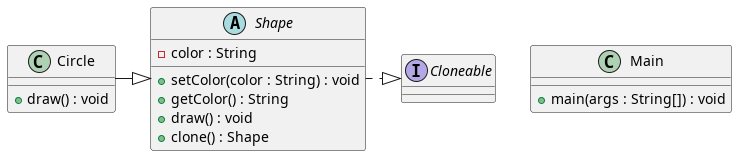
\includegraphics[width=.9\textwidth]{../figures/out/prototype.png}
 	\caption{Prototype Pattern}
 	\label{fig:prototype}
\end{figure}

\subsection{Contoh Shape}

\begin{lstlisting}[style=JavaStyle, caption={Implementasi Prototype pada Kelas Shape}, label={lst:prototype-shape}]
public abstract class Shape implements Cloneable {
	protected String color;
	
	public void setColor(String color) {
		this.color = color;
	}
	
	public String getColor() {
		return color;
	}
	
	public abstract void draw();
	
	@Override
	public Shape clone() {
		try {
			return (Shape) super.clone();
		} catch (CloneNotSupportedException e) {
			throw new AssertionError();
		}
	}
}
\end{lstlisting}

Kode di atas mengimplementasikan pola \textit{Prototype} melalui kelas abstrak \texttt{Shape}, yang dirancang untuk dapat dikloning. Kelas ini mendeklarasikan satu atribut \texttt{color} bertipe \texttt{String} yang dapat diatur melalui metode \texttt{setColor()} dan diakses melalui metode \texttt{getColor()}. 

Kelas \texttt{Shape} juga mendefinisikan metode abstrak \texttt{draw()}, yang akan diimplementasikan secara spesifik oleh subclass untuk menggambarkan perilaku menggambar bentuk tertentu. Dengan cara ini, \texttt{Shape} hanya mendefinisikan struktur dasar dan kontrak fungsional, sementara detail implementasi diserahkan kepada kelas konkret yang mewarisinya.

Poin penting dari implementasi ini adalah metode \texttt{clone()} yang di-\texttt{override}. Metode ini menggunakan mekanisme \texttt{super.clone()} dari kelas induk \texttt{Object} untuk membuat salinan objek \texttt{Shape}. Karena Java mewajibkan bahwa objek yang ingin dikloning harus mengimplementasikan antarmuka \texttt{Cloneable}, kelas \texttt{Shape} juga mendeklarasikan bahwa ia mengimplementasikan \texttt{Cloneable}. Jika proses cloning gagal (misalnya, jika terjadi \texttt{CloneNotSupportedException}), maka sebuah \texttt{AssertionError} akan dilemparkan untuk menandai kegagalan serius.

Dengan pola ini, setiap subclass dari \texttt{Shape} secara otomatis akan memiliki kemampuan untuk dikloning tanpa harus menulis ulang logika cloning, selama semua atribut yang digunakan adalah tipe yang mendukung \textit{shallow copy}. Pendekatan ini mempercepat pembuatan salinan objek dengan konfigurasi yang serupa, serta menjaga konsistensi antar objek yang dibangun berdasarkan prototipe yang sama.


\begin{lstlisting}[style=JavaStyle, caption={Kelas Circle yang Mengimplementasikan Shape}, label={lst:prototype-circle}]
public class Circle extends Shape {
	@Override
	public void draw() {
		System.out.println("Drawing a " + color + " circle.");
	}
}
\end{lstlisting}

Kode di atas mendefinisikan kelas \texttt{Circle} sebagai subclass dari kelas abstrak \texttt{Shape}. Kelas ini mengimplementasikan metode abstrak \texttt{draw()} yang didefinisikan di \texttt{Shape}. 

Dalam implementasi metode \texttt{draw()}, kelas \texttt{Circle} menampilkan pesan ke konsol yang menunjukkan bahwa sebuah lingkaran (\texttt{circle}) sedang digambar, disertai dengan warna yang disimpan dalam atribut \texttt{color}. Nilai warna ini diatur menggunakan metode \texttt{setColor()} yang diwarisi dari kelas induk \texttt{Shape}.

Karena \texttt{Circle} mewarisi kemampuan \texttt{clone()} dari \texttt{Shape}, objek \texttt{Circle} dapat dikloning tanpa perlu mengimplementasikan logika cloning secara eksplisit di dalam kelas ini. Dengan demikian, pola \textit{Prototype} dapat diterapkan untuk membuat salinan objek \texttt{Circle} dengan konfigurasi warna yang sama atau dimodifikasi sesuai kebutuhan. 

Implementasi ini memperlihatkan bagaimana subclass cukup fokus pada perilaku spesifiknya, sementara mekanisme cloning dan atribut umum sudah ditangani oleh kelas induk, sehingga mendukung prinsip pemisahan tanggung jawab dan mempermudah perluasan sistem di masa depan.

\begin{lstlisting}[style=JavaStyle, caption={Penggunaan Pola Prototype untuk Mengkloning Shape}, label={lst:prototype-main}]
public class Main {
	public static void main(String[] args) {
		Circle originalCircle = new Circle();
		originalCircle.setColor("Red");
		
		Circle clonedCircle = (Circle) originalCircle.clone();
		clonedCircle.setColor("Blue");
		
		originalCircle.draw();   // Output: Drawing a Red circle.
		clonedCircle.draw();     // Output: Drawing a Blue circle.
	}
}
\end{lstlisting}

Kode di atas menunjukkan contoh penggunaan pola \textit{Prototype} untuk membuat salinan objek \texttt{Shape} secara dinamis. Pertama-tama, dibuat sebuah objek \texttt{originalCircle} dari kelas \texttt{Circle} dan diatur warnanya menjadi "Red" menggunakan metode \texttt{setColor()}. 

Objek ini kemudian dikloning menjadi \texttt{clonedCircle} menggunakan metode \texttt{clone()}, dan warna dari salinan tersebut diubah menjadi "Blue" tanpa mempengaruhi objek \texttt{originalCircle}.

Pemanggilan metode \texttt{draw()} pada kedua objek menampilkan lingkaran dengan warna yang berbeda, yaitu "Red" untuk objek asli dan "Blue" untuk objek hasil cloning. Hasil ini menunjukkan bahwa cloning berhasil menciptakan objek baru yang dapat dimodifikasi secara independen dari objek sumber.

Dengan pola \textit{Prototype}, proses pembuatan objek baru menjadi lebih fleksibel dan efisien, terutama ketika struktur objek yang sama perlu direplikasi dengan sedikit perubahan konfigurasi. Pendekatan ini juga membantu menjaga konsistensi struktur internal sambil tetap memungkinkan variasi eksternal pada setiap instansi.



\subsection{Contoh Report}

\begin{lstlisting}[style=JavaStyle, caption={Implementasi Prototype pada Kelas Report}, label={lst:prototype-report}]
public class Report implements Cloneable {
	private String title;
	private String content;
	
	public Report(String title, String content) {
		this.title = title;
		this.content = content;
	}
	
	public void setTitle(String title) {
		this.title = title;
	}
	
	public void setContent(String content) {
		this.content = content;
	}
	
	public void printReport() {
		System.out.println("Title: " + title);
		System.out.println("Content: " + content);
	}
	
	@Override
	public Report clone() {
		try {
			return (Report) super.clone();
		} catch (CloneNotSupportedException e) {
			throw new AssertionError();
		}
	}
}
\end{lstlisting}

Kode di atas mengimplementasikan pola \textit{Prototype} pada kelas \texttt{Report}, yang merepresentasikan sebuah dokumen laporan dengan dua atribut utama: \texttt{title} dan \texttt{content}. Kelas ini menyediakan konstruktor untuk menginisialisasi kedua atribut tersebut, serta metode \texttt{setTitle()} dan \texttt{setContent()} untuk memungkinkan perubahan nilai setelah objek dibuat.

Metode \texttt{printReport()} digunakan untuk menampilkan isi laporan ke konsol, dengan mencetak nilai dari \texttt{title} dan \texttt{content}. 

Bagian penting dari implementasi ini adalah metode \texttt{clone()} yang di-\texttt{override} dari kelas \texttt{Object}. Metode ini memanfaatkan mekanisme \texttt{super.clone()} untuk menghasilkan salinan baru dari objek \texttt{Report}. Karena \texttt{Report} mengimplementasikan antarmuka \texttt{Cloneable}, proses cloning dapat dilakukan tanpa error, dan jika cloning gagal, maka \texttt{AssertionError} akan dilemparkan sebagai bentuk penanganan kegagalan yang tegas.

Dengan pendekatan ini, objek \texttt{Report} dapat dikloning dengan cepat, memungkinkan penciptaan dokumen baru berdasarkan template yang sudah ada tanpa perlu membuat objek baru dari awal. Ini sangat berguna dalam konteks sistem yang membutuhkan banyak variasi laporan berdasarkan struktur dasar yang serupa.

\begin{lstlisting}[style=JavaStyle, caption={Penggunaan Prototype untuk Mengkloning Report}, label={lst:prototype-report-main}]
public class Main {
	public static void main(String[] args) {
		Report monthlyReport = new Report("Monthly Report", "Summary of activities...");
		
		Report clonedReport = monthlyReport.clone();
		clonedReport.setTitle("Monthly Report - Copy");
		
		monthlyReport.printReport();
		System.out.println();
		clonedReport.printReport();
	}
}
\end{lstlisting}

Kode di atas memperlihatkan penggunaan pola \textit{Prototype} untuk mengkloning objek \texttt{Report}. Pertama-tama, dibuat objek \texttt{monthlyReport} dengan judul "Monthly Report" dan isi "Summary of activities...". 

Objek ini kemudian dikloning menggunakan metode \texttt{clone()} untuk membuat objek baru bernama \texttt{clonedReport}. Setelah cloning, judul pada \texttt{clonedReport} diubah menjadi "Monthly Report - Copy" menggunakan metode \texttt{setTitle()}, sementara isi laporan tetap sama dengan objek asli.

Metode \texttt{printReport()} dipanggil pada kedua objek untuk menampilkan isi masing-masing laporan ke konsol. Pemisahan isi antara \texttt{monthlyReport} dan \texttt{clonedReport} menunjukkan bahwa perubahan pada objek hasil cloning tidak mempengaruhi objek sumber, sehingga masing-masing objek adapt dimodifikasi secara independen.

Contoh ini menggambarkan kekuatan pola \textit{Prototype} dalam mempercepat penciptaan objek baru berdasarkan template yang ada, sekaligus memungkinkan penyesuaian ringan tanpa perlu membangun objek dari awal.

\section{Pola Kreasi: Dependency Injection}

\subsection{Tujuan dan Konteks Penggunaan}

Pola \textit{Dependency Injection} (DI) merupakan pola kreasi yang bertujuan untuk mengelola ketergantungan antar objek dalam sebuah sistem perangkat lunak dengan cara menyerahkan pembuatan dan penyediaan objek ketergantungan (\textit{dependencies}) kepada pihak luar, bukan dengan membuatnya langsung di dalam kelas yang menggunakannya. Dengan pendekatan ini, setiap objek tidak bertanggung jawab untuk membuat atau mengatur sendiri ketergantungan yang dibutuhkannya, melainkan menerima ketergantungan tersebut dari luar melalui berbagai cara seperti konstruktor, metode, atau properti.

Tujuan utama dari penerapan pola Dependency Injection adalah untuk:
\begin{itemize}
\item Mengurangi keterikatan (\textit{tight coupling}) antara kelas, sehingga kode menjadi lebih fleksibel, mudah diuji, dan lebih mudah untuk dikembangkan.
\item Meningkatkan kemampuan sistem untuk beradaptasi terhadap perubahan, karena ketergantungan dapat diganti dengan mudah tanpa memodifikasi kelas pengguna.
\item Mendukung prinsip desain perangkat lunak seperti \textit{Dependency Inversion Principle} (DIP), di mana kode bergantung pada abstraksi, bukan pada implementasi konkret.
\end{itemize}

Pola Dependency Injection umumnya digunakan dalam aplikasi berskala besar di mana pengelolaan ketergantungan menjadi kompleks. Dengan menggunakan pola ini, komponen-komponen dalam sistem menjadi lebih modular, dapat dipertukarkan, dan dapat diuji secara terpisah menggunakan teknik seperti \textit{mocking} atau \textit{stubbing}.

Ada beberapa cara umum untuk menerapkan Dependency Injection dalam sistem perangkat lunak:
\begin{itemize}
\item \textbf{Constructor Injection}: Ketergantungan disuntikkan melalui parameter konstruktor saat objek dibuat.
\item \textbf{Setter Injection}: Ketergantungan disuntikkan melalui metode \texttt{setter} setelah objek dibuat.
\item \textbf{Interface Injection}: Objek menerima ketergantungan melalui metode yang ditentukan oleh sebuah antarmuka.
\end{itemize}

Penerapan pola ini dapat dilakukan secara manual, atau dengan bantuan kerangka kerja (framework) khusus seperti Spring Framework di Java, yang menyediakan mekanisme otomatis untuk mengelola siklus hidup objek dan injeksi ketergantungan.

\subsection{Contoh Kasus Penggunaan}

Salah satu contoh umum penggunaan pola \textit{Dependency Injection} adalah pada pengembangan aplikasi berbasis layanan, seperti layanan pembayaran dalam sebuah sistem e-commerce. Misalnya, sebuah kelas \texttt{OrderService} membutuhkan objek \texttt{PaymentProcessor} untuk memproses pembayaran. Daripada membuat instansi \texttt{PaymentProcessor} secara langsung di dalam \texttt{OrderService}, objek tersebut disuntikkan dari luar. Dengan demikian, \texttt{OrderService} tidak bergantung pada implementasi konkret dan dapat dengan mudah menggunakan berbagai jenis \texttt{PaymentProcessor}, seperti \texttt{CreditCardProcessor} atau \texttt{PayPalProcessor}, tanpa perubahan pada kode inti.

Contoh lainnya adalah dalam pembuatan sistem logging. Sebuah kelas \texttt{Application} dapat menerima objek \texttt{Logger} melalui constructor injection. Jika di masa depan ada kebutuhan untuk mengganti sistem logging dari file-based logger ke cloud-based logger, perubahan dapat dilakukan hanya dengan menyuntikkan objek logger baru tanpa memodifikasi kode kelas \texttt{Application}.

Dalam konteks pengujian unit (\textit{unit testing}), Dependency Injection juga sangat berguna. Misalnya, sebuah kelas yang bergantung pada akses database dapat diuji dengan menyuntikkan objek \texttt{MockDatabase} alih-alih database nyata. Ini memungkinkan pengujian dilakukan dengan cepat, konsisten, dan tanpa bergantung pada infrastruktur eksternal.

Dalam pengembangan aplikasi skala besar, Dependency Injection sering dikelola secara otomatis oleh framework seperti Spring di Java atau Dagger di Android. Framework ini menyediakan kontainer yang bertugas mengelola siklus hidup objek, menyuntikkan ketergantungan yang diperlukan, dan menjaga struktur sistem tetap bersih serta modular.

Dengan menggunakan Dependency Injection, sistem menjadi lebih fleksibel dalam mengelola variasi implementasi, lebih mudah diuji, dan lebih tahan terhadap perubahan, sehingga mendukung prinsip desain perangkat lunak modern yang berorientasi pada modularitas dan keterpisahan tanggung jawab.


\subsection{Kelebihan dan Kekurangan}

\textbf{Kelebihan:}
\begin{itemize}
\item \textbf{Mengurangi keterikatan antar kelas:} Dengan Dependency Injection, kelas tidak perlu mengetahui detail tentang bagaimana ketergantungan dibuat atau diatur. Ini memungkinkan komponen menjadi lebih modular dan lebih mudah dipertukarkan.

\item \textbf{Meningkatkan keterujian:} Karena ketergantungan dapat disuntikkan dari luar, pengujian unit menjadi lebih sederhana. Objek-objek tiruan (\textit{mock}) dapat dengan mudah digunakan untuk menggantikan implementasi nyata selama pengujian.

\item \textbf{Mendukung prinsip SOLID:} Dependency Injection secara langsung mendukung prinsip \textit{Dependency Inversion Principle} (DIP) dalam SOLID, di mana kelas bergantung pada abstraksi daripada implementasi konkret.

\item \textbf{Mempermudah pengelolaan ketergantungan:} Dalam sistem besar, jumlah objek dan hubungan ketergantungan antar objek dapat menjadi kompleks. Dengan menggunakan pola ini, pengelolaan ketergantungan menjadi lebih terstruktur dan sistematis, terutama dengan bantuan framework.

\item \textbf{Meningkatkan fleksibilitas dan skalabilitas:} Sistem menjadi lebih adaptif terhadap perubahan. Ketergantungan baru dapat diperkenalkan atau diganti tanpa perlu memodifikasi kode kelas utama.
\end{itemize}

\textbf{Kekurangan:}
\begin{itemize}
\item \textbf{Menambah kompleksitas awal:} Untuk proyek kecil, penggunaan Dependency Injection dapat terasa berlebihan karena menambah lapisan tambahan dan memerlukan pengaturan struktur yang lebih kompleks.

\item \textbf{Membutuhkan pemahaman yang lebih tinggi:} Pengembang perlu memahami prinsip kerja Dependency Injection dan bagaimana mengonfigurasi ketergantungan, terutama saat menggunakan framework otomatis seperti Spring.

\item \textbf{Sulit dilacak secara manual:} Jika Dependency Injection dikelola tanpa framework, pengaturan dan pengelolaan semua ketergantungan secara manual dapat menjadi sulit dilacak, terutama dalam sistem yang sangat besar.

\item \textbf{Peningkatan waktu inisialisasi:} Pada sistem dengan banyak ketergantungan yang kompleks, proses pembuatan dan injeksi objek di awal program dapat memperlambat waktu startup aplikasi.

\item \textbf{Ketergantungan pada framework:} Dalam banyak kasus, sistem yang menggunakan Dependency Injection bergantung pada framework pihak ketiga, yang menambah dependensi eksternal dan perlu dipertimbangkan dalam aspek pemeliharaan dan pembaruan jangka panjang.
\end{itemize}


\subsection{Implementasi dalam Java}

Implementasi pola \textit{Dependency Injection} dalam Java dapat divisualisasikan seperti yang ditunjukkan pada Gambar~\ref{fig:dependency-injection}. Diagram tersebut memperlihatkan bagaimana sebuah objek ketergantungan tidak dibuat langsung oleh kelas pengguna, melainkan disediakan dari luar melalui mekanisme injeksi. Dengan pendekatan ini, kelas pengguna hanya bergantung pada antarmuka atau abstraksi, bukan pada implementasi konkret. Hal ini meningkatkan fleksibilitas, keterujian, dan memungkinkan sistem untuk lebih mudah beradaptasi terhadap perubahan. Berikut ini adalah contoh implementasi kode dalam Java yang menerapkan pola Dependency Injection menggunakan teknik constructor injection.

\begin{figure}[h]
 	\centering
 	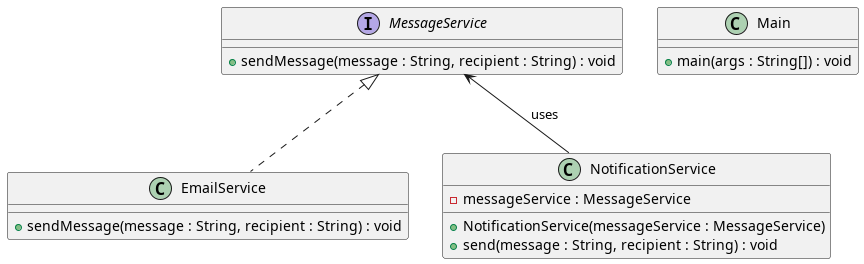
\includegraphics[width=.9\textwidth]{../figures/out/dependency_injection.png}
 	\caption{Dependency Injection}
 	\label{fig:dependency-injection}
\end{figure}


\subsection{Contoh Message Service}

\begin{lstlisting}[style=JavaStyle, caption={Implementasi Dependency Injection dengan Constructor Injection}, label={lst:di-constructor}]
public interface MessageService {
	void sendMessage(String message, String recipient);
}
\end{lstlisting}

Kode di atas mendefinisikan antarmuka \texttt{MessageService} yang berfungsi sebagai kontrak untuk layanan pengiriman pesan. Antarmuka ini mendeklarasikan satu metode \texttt{sendMessage()} yang menerima dua parameter: \texttt{message} dan \texttt{recipient}, keduanya bertipe \texttt{String}. 

Dengan mendefinisikan kontrak ini, sistem dapat memiliki berbagai implementasi konkret dari \texttt{MessageService} tanpa bergantung pada kelas tertentu. Kelas-klas lain yang membutuhkan layanan pengiriman pesan cukup bergantung pada antarmuka ini, sehingga mendukung prinsip \textit{Dependency Inversion} dan memperkuat modularitas sistem.

Antarmuka ini menjadi dasar bagi penerapan pola \textit{Dependency Injection}, di mana ketergantungan terhadap layanan pesan disuntikkan ke dalam kelas pengguna tanpa menciptakan ketergantungan langsung terhadap implementasi spesifik.


\begin{lstlisting}[style=JavaStyle, caption={Implementasi Konkret dari MessageService}, label={lst:di-email-service}]
public class EmailService implements MessageService {
	@Override
	public void sendMessage(String message, String recipient) {
		System.out.println("Email sent to " + recipient + " with message: " + message);
	}
}
\end{lstlisting}

Kode di atas mengimplementasikan antarmuka \texttt{MessageService} melalui kelas \texttt{EmailService}. Kelas ini memberikan implementasi konkret untuk metode \texttt{sendMessage()}, di mana pesan akan dikirimkan ke penerima melalui mekanisme email. Dalam contoh ini, pengiriman email disimulasikan dengan mencetak pesan ke konsol menggunakan \texttt{System.out.println()}.

Dengan menerapkan kontrak dari \texttt{MessageService}, kelas \texttt{EmailService} dapat disuntikkan ke dalam komponen lain seperti \texttt{NotificationService} tanpa menyebabkan ketergantungan langsung terhadap implementasi spesifik. Jika di masa depan diperlukan layanan lain seperti \texttt{SMSService} atau \texttt{PushNotificationService}, penggantian implementasi dapat dilakukan dengan mudah tanpa perlu mengubah kode kelas klien.

Kelas ini memperlihatkan bagaimana Dependency Injection memisahkan tanggung jawab antara mendefinisikan kebutuhan layanan (melalui antarmuka) dan menyediakan implementasi layanan tersebut.


\begin{lstlisting}[style=JavaStyle, caption={Kelas Client yang Menerima Ketergantungan Melalui Konstruktor}, label={lst:di-client}]
public class NotificationService {
	private MessageService messageService;
	
	public NotificationService(MessageService messageService) {
		this.messageService = messageService;
	}
	
	public void send(String message, String recipient) {
		messageService.sendMessage(message, recipient);
	}
}
\end{lstlisting}

Kode di atas mendefinisikan kelas \texttt{NotificationService} yang berperan sebagai klien yang menggunakan layanan pengiriman pesan. Kelas ini memiliki satu atribut privat bertipe \texttt{MessageService}, yang diatur melalui konstruktor menggunakan pola \textit{constructor injection}. 

Dengan pendekatan ini, objek \texttt{NotificationService} tidak membuat atau menginisialisasi sendiri objek \texttt{MessageService}, melainkan menerima instansinya dari luar pada saat pembuatan objek. Hal ini mendukung prinsip \textit{Dependency Inversion}, karena \texttt{NotificationService} hanya bergantung pada abstraksi, bukan pada implementasi konkret seperti \texttt{EmailService}.

Metode \texttt{send()} digunakan untuk mengirimkan pesan kepada penerima tertentu dengan memanggil metode \texttt{sendMessage()} dari objek \texttt{MessageService} yang sudah disuntikkan. Dengan struktur ini, \texttt{NotificationService} menjadi fleksibel dan mudah diuji, karena dapat menerima berbagai implementasi \texttt{MessageService} sesuai kebutuhan, baik implementasi nyata maupun objek tiruan (\textit{mock}) saat pengujian.


\begin{lstlisting}[style=JavaStyle, caption={Kode Main untuk Menjalankan Dependency Injection}, label={lst:di-main}]
public class Main {
	public static void main(String[] args) {
		// Injeksi ketergantungan secara manual
		MessageService service = new EmailService();
		NotificationService notification = new NotificationService(service);
		
		notification.send("Hello, Dependency Injection!", "user@example.com");
	}
}
\end{lstlisting}

Kode di atas memperlihatkan bagaimana Dependency Injection diterapkan secara manual di dalam metode \texttt{main()}. Pertama-tama, dibuat sebuah instansi \texttt{EmailService} yang merupakan implementasi konkret dari antarmuka \texttt{MessageService}. Objek ini kemudian disuntikkan ke dalam konstruktor kelas \texttt{NotificationService}, sehingga objek \texttt{NotificationService} tidak perlu membuat atau mengetahui detail implementasi layanan pesan yang digunakannya.

Dengan struktur ini, \texttt{NotificationService} cukup berinteraksi dengan antarmuka \texttt{MessageService}, tanpa ketergantungan langsung terhadap kelas \texttt{EmailService}. Setelah injeksi ketergantungan dilakukan, metode \texttt{send()} dipanggil untuk mengirimkan pesan "Hello, Dependency Injection!" ke penerima "user@example.com".

Contoh ini menggambarkan penerapan sederhana dari konsep Dependency Injection, di mana ketergantungan dikelola secara eksternal, meningkatkan fleksibilitas sistem, dan mendukung prinsip desain perangkat lunak yang baik.

\subsection{Contoh Weather}

\begin{lstlisting}[style=JavaStyle, caption={Antarmuka WeatherService untuk Memberikan Informasi Cuaca}, label={lst:di-weather-service}]
public interface WeatherService {
	String getWeatherUpdate();
}
\end{lstlisting}

Kode di atas mendefinisikan antarmuka \texttt{WeatherService} yang berfungsi sebagai kontrak untuk layanan penyedia informasi cuaca. Antarmuka ini mendeklarasikan satu metode \texttt{getWeatherUpdate()} yang mengembalikan sebuah nilai bertipe \texttt{String}. 

Dengan adanya antarmuka ini, kelas-kelas yang membutuhkan data cuaca tidak perlu mengetahui bagaimana data tersebut diperoleh atau dari layanan mana data itu berasal. Mereka cukup bergantung pada kontrak yang sudah ditentukan oleh \texttt{WeatherService}. Pendekatan ini mendorong penerapan prinsip \textit{Dependency Inversion}, di mana kode klien bergantung pada abstraksi, bukan pada implementasi konkret.

Antarmuka ini menjadi landasan bagi penerapan pola \textit{Dependency Injection}, karena memungkinkan implementasi layanan cuaca yang berbeda-beda disuntikkan ke dalam klien tanpa perlu mengubah kode klien tersebut.


\begin{lstlisting}[style=JavaStyle, caption={Implementasi Konkret dari WeatherService}, label={lst:di-weather-api}]
public class WeatherAPIService implements WeatherService {
	@Override
	public String getWeatherUpdate() {
		return "Today's weather: Sunny, 30 degrees Celsius.";
	}
}
\end{lstlisting}


Kode di atas mengimplementasikan antarmuka \texttt{WeatherService} melalui kelas \texttt{WeatherAPIService}. Kelas ini memberikan implementasi konkret untuk metode \texttt{getWeatherUpdate()}, di mana dalam contoh ini metode tersebut mengembalikan informasi cuaca berupa teks "Today's weather: Sunny, 30°C.".

Dengan mengimplementasikan kontrak \texttt{WeatherService}, kelas ini dapat digunakan oleh berbagai klien tanpa menyebabkan ketergantungan langsung terhadap detail implementasi. Jika di masa depan ingin mengganti sumber data cuaca, seperti mengambil data dari API eksternal atau basis data lokal, perubahan dapat dilakukan dengan membuat implementasi baru dari \texttt{WeatherService} tanpa memodifikasi kode klien.

Kelas ini mendemonstrasikan prinsip pemisahan tanggung jawab, di mana \texttt{WeatherAPIService} hanya fokus pada penyediaan data cuaca, sementara logika penggunaan data tersebut ditangani oleh klien seperti \texttt{WeatherReporter}.


\begin{lstlisting}[style=JavaStyle, caption={Kelas Client yang Menggunakan Setter untuk Dependency Injection}, label={lst:di-weather-client-setter}]
public class WeatherReporter {
	private WeatherService weatherService;
	
	public WeatherReporter() {
		// Konstruktor default tanpa parameter
	}
	
	public void setWeatherService(WeatherService weatherService) {
		this.weatherService = weatherService;
	}
	
	public void report() {
		if (weatherService != null) {
			System.out.println(weatherService.getWeatherUpdate());
		} else {
			System.out.println("WeatherService is not available.");
		}
	}
}
\end{lstlisting}

Kode di atas mendefinisikan kelas \texttt{WeatherReporter} yang berfungsi sebagai klien yang menerima ketergantungan terhadap layanan cuaca melalui \textit{setter injection}. Kelas ini memiliki atribut privat bertipe \texttt{WeatherService} yang diatur melalui metode \texttt{setWeatherService()}.

Konstruktor \texttt{WeatherReporter} tidak menerima parameter apa pun, sehingga objek dapat dibuat tanpa ketergantungan sejak awal. Ketergantungan kemudian disuntikkan setelah objek dibuat dengan memanggil metode \texttt{setWeatherService()}. Pendekatan ini memberikan fleksibilitas, terutama jika ketergantungan perlu disiapkan atau diganti setelah instansiasi.

Metode \texttt{report()} digunakan untuk menampilkan informasi cuaca. Di dalam metode ini terdapat pemeriksaan apakah \texttt{weatherService} sudah tersedia sebelum digunakan, untuk menghindari terjadinya \texttt{NullPointerException}.

Implementasi ini mendemonstrasikan pola \textit{Setter Dependency Injection}, di mana ketergantungan disuntikkan melalui metode \texttt{setter} alih-alih melalui konstruktor, sehingga memungkinkan penundaan atau penggantian ketergantungan di waktu yang lebih fleksibel.

\begin{lstlisting}[style=JavaStyle, caption={Kode Main untuk Menjalankan Setter Dependency Injection pada Weather Reporter}, label={lst:di-weather-main-setter}]
public class Main {
	public static void main(String[] args) {
		// Membuat objek layanan
		WeatherService service = new WeatherAPIService();
		
		// Membuat klien dan melakukan setter injection
		WeatherReporter reporter = new WeatherReporter();
		reporter.setWeatherService(service);
		
		reporter.report();
	}
}
\end{lstlisting}

Kode di atas memperlihatkan bagaimana pola \textit{Setter Dependency Injection} diterapkan untuk menghubungkan layanan cuaca dengan klien \texttt{WeatherReporter}. Pertama-tama, dibuat objek \texttt{WeatherAPIService} yang merupakan implementasi konkret dari antarmuka \texttt{WeatherService}. 

Kemudian, dibuat instansi \texttt{WeatherReporter} menggunakan konstruktor default tanpa parameter. Setelah objek \texttt{WeatherReporter} dibuat, layanan cuaca disuntikkan ke dalamnya melalui metode \texttt{setWeatherService()}. 

Setelah ketergantungan diatur, metode \texttt{report()} dipanggil untuk mengambil dan menampilkan informasi cuaca yang disediakan oleh \texttt{WeatherAPIService}. 

Dengan pendekatan ini, pembuatan dan penyuntikan ketergantungan dipisahkan dari pembuatan objek klien, memberikan fleksibilitas lebih dalam mengelola ketergantungan, seperti mengganti implementasi layanan tanpa harus memodifikasi konstruktor atau logika internal kelas \texttt{WeatherReporter}.


\section{Kesimpulan}

Pada bab ini telah dibahas tiga pola kreasi penting dalam pengembangan perangkat lunak berorientasi objek, yaitu \textit{Builder}, \textit{Prototype}, dan \textit{Dependency Injection}. Pola \textit{Builder} menawarkan pendekatan bertahap dalam membangun objek kompleks dengan banyak atribut opsional, meningkatkan keterbacaan dan fleksibilitas kode. Pola \textit{Prototype} memfasilitasi penciptaan objek baru melalui cloning, menghemat waktu dan sumber daya, terutama saat berhadapan dengan struktur objek yang kompleks. Sementara itu, pola \textit{Dependency Injection} berfokus pada pengelolaan ketergantungan antar objek dengan menyuntikkan dependensi dari luar, sehingga mendukung modularitas, keterujian, dan prinsip desain yang baik seperti Dependency Inversion Principle.

Penerapan ketiga pola ini secara tepat memungkinkan sistem perangkat lunak menjadi lebih fleksibel, scalable, dan mudah dipelihara. Pola \textit{Builder} sangat berguna dalam skenario pembuatan objek dengan banyak konfigurasi, \textit{Prototype} efektif untuk replikasi cepat objek kompleks, dan \textit{Dependency Injection} memperkuat arsitektur sistem dengan mengurangi keterikatan antar komponen. Pemahaman mendalam terhadap karakteristik, kelebihan, dan kekurangan masing-masing pola sangat penting untuk memilih pola yang paling sesuai dengan kebutuhan arsitektur dan konteks pengembangan yang dihadapi.
